\documentclass[12pt]{article}
\usepackage{url,graphicx,tabularx,array,geometry}
\usepackage[utf8]{inputenc}
\usepackage{amsmath}
\setlength{\parskip}{1ex} %--skip lines between paragraphs
\setlength{\parindent}{0pt} %--don't indent paragraphs
\usepackage{listings}
\usepackage{pgf}
\usepackage{tikz}
\usetikzlibrary{arrows,automata}

%-- Commands for header
\renewcommand{\title}[1]{\textbf{#1}\\}
\renewcommand{\line}{\begin{tabularx}{\textwidth}{X>{\raggedleft}X}\hline\\\end{tabularx}\\[-0.5cm]}
\newcommand{\leftright}[2]{\begin{tabularx}{\textwidth}{X>{\raggedleft}X}#1%
& #2\\\end{tabularx}\\[-0.5cm]}

%\linespread{2} %-- Uncomment for Double Space
\begin{document}

\title{Robotics Project  Autumn 2013}
\line
\leftright{\today}{Alexander Rüedlinger, 08-129-710, Group 01} %-- left and right positions in the header
\section*{Series 5}
\paragraph{Remark} 
Because I don't know what is expected in this exercise I decided to write a report with problems we encountered and the questions we had in mind.

\paragraph{a)} Done! Me and my team-mate we went two times to the lab.
However, we've found out that the aseba studio version on the ubuntu machines are not compatible with the version installed on our notebooks.

For example we had to adapt the following lines:
\begin{lstlisting}
speed.left -> leftSpeed
speed.right -> rightSpeed
\end{lstlisting}

Besides that the behaviour of the epucks compared to the simulator is totally different!
\subparagraph{Our conclusion}
For testing an aseba file we had to create two files. One for the simulator and one for the physical arena. This can be an error prone task and violates the "Don't repeat yourself principle". It is necessary to test each line of code in the physical arena because the conditions and the environment are to idealistic in the simulator (sensor values, e.g. color values).

\paragraph{b)}
\subparagraph{State machine}
As introduced in the lecture we've applied the state machine concept to solve this exercise.
As required we wrote two subroutines called lover and explorer. The transition between these two states is done by means of timer routine which changes the states after a specific time period.
\subparagraph{Pair programming / code review}
We did some pair programming and code review. However, we could not agree on which code snippet is better in order to switch between states (in subroutine timer):

\begin{lstlisting}
if state == EXPLORER then
	state = LOVER
else
	state = EXPLORER
end
\end{lstlisting}
versus
\begin{lstlisting}
state = 1 - state
\end{lstlisting}
\begin{enumerate}
\item 1. version 
	\begin{enumerate}
		\item more explicit
		\item readable
	\end{enumerate}
\item 2. version
	\begin{enumerate}
		\item less code
		\item less readable
	\end{enumerate}
\end{enumerate}

In my opinion the first version is better as a future maintainer of this code.
My colleague in contrast prefers the second version.
\paragraph{Because we all like graphs...}
What our code does can be described by the following simple state machine:
\begin{figure}[!htb]
\centering

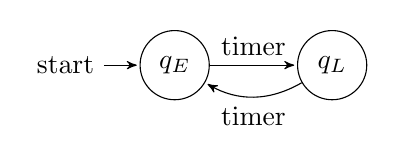
\begin{tikzpicture}[>=stealth',shorten >=1pt,auto,node distance=2cm]
  \node[initial,state] (S)      {$q_E$};
  \node[state]         (q1) [right of=S]  {$q_L$};
 
 
  \path[->] (S) 
             edge              node {timer} (q1)
        (q1) edge [bend left]  node {timer} (S);
\end{tikzpicture}
\end{figure}

($q_L$ : lover state, $q_E$ : explorer state)

\end{document}
